\documentclass[11pt]{article}
\usepackage[utf8]{inputenc}
\usepackage[T1]{fontenc}
\usepackage{amsmath}
\usepackage{amsfonts}
\usepackage{amssymb}
\usepackage[version=4]{mhchem}
\usepackage{stmaryrd}
\usepackage{graphicx}
\usepackage[export]{adjustbox}
\graphicspath{ {./images/} }

\begin{document}
Mechanics of and Motivations for an Arbitrage CDO

This lesson begins with a simplified example of an arbitrage CDO.

\section*{Example of an Arbitrage CDO}
Assume a money manager establishes an arbitrage CDO to invest in high-yield bonds. The trust has a life of five years and raises $\$ 500$ million by selling (issuing) tranches of securities. For simplicity, assume that there are only three tranches, although in practice there can be numerous tranches. The security tranches issued by the trust are divided by credit rating. The most senior tranche, Tranche A, is a fixed-income tranche that is issued with the highest priority against the trust collateral. This highly rated debt will have a lower coupon, lower yield, lower expected return, and lower volatility than the collateral pool.

The second, or mezzanine, tranche, Tranche B, has lower seniority than Tranche A but enjoys the subordination of the equity tranche that will bear first losses. The credit rating of Tranche B may be only slightly higher than or roughly similar to the average high-yield bond owned by the CDO trust. The final tranche, Tranche C, is subordinated to the other two CDO tranches. For this tranche, the risk is the highest. This equity tranche also collects any residual income generated by the CDO collateral.

The next exhibit illustrates this arbitrage CDO trust. The money manager assembles a $\$ 450$ million portfolio of high-yield bonds, with credit ratings of the underlying issuers equal to BB. The bonds pay an average annual coupon of $9 \%$ and have a face value of $\$ 500$ million and a current market value of $\$ 450$ million. In addition, the money manager charges an annual management fee of 50 basis points for managing the market value of the trust's assets: 50 basis points $\times \$ 500$ million $=\$ 2.5$ million. Last, suppose there are annual expenses totaling $\$ 1.5$ million that include such fees as $\$ 250,000$ for the trustee to oversee the indenture clauses of the CDO notes. As illustrated in An Arbitrage CDO Structure exhibit, the CDO trust also buys a $\$ 50$ million five-year U.S. Treasury note at an annual coupon rate of $6 \%$.

\begin{center}
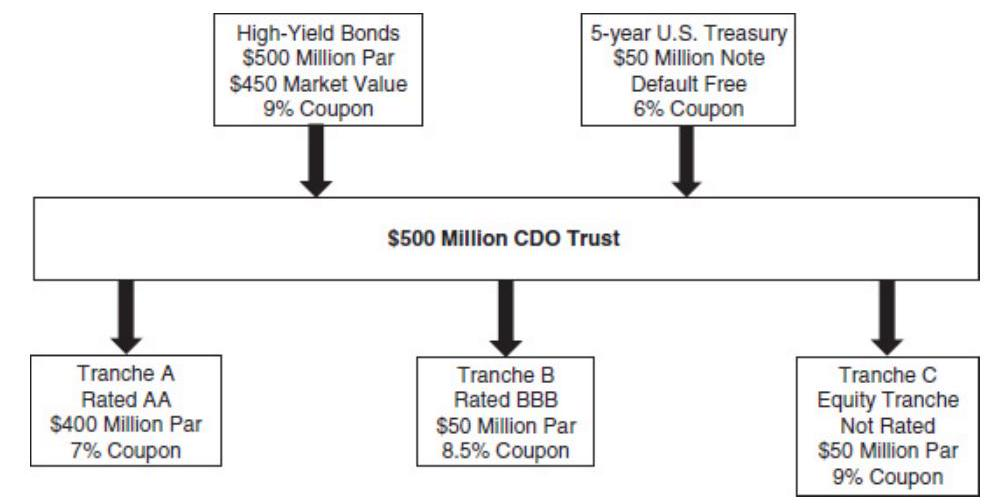
\includegraphics[max width=\textwidth]{2024_04_10_bea18d3cfa917e559286g-2}
\end{center}

\section*{An Arbitrage CDO Structure}
\section*{Three Tranches and Their Priorities}
The Treasury note is used to provide credit protection to Tranche A and helps allow for an AA credit rating to the senior tranche, along with the diversification and the subordination of the other tranches. Tranche A has a $\$ 400$ million face value and a coupon of $7 \%$, and, as an AA-rated security, it is easily sold to institutions seeking securities with investment grade ratings. The investors in Tranche A receive a higher yield than that given by U.S. Treasuries because the CDO has credit risk and perhaps merits a complexity premium.

The second tranche has a face value of $\$ 50$ million and a stated coupon of $8.5 \%$ and is rated BBB. This tranche has a higher rating than the underlying high-yield bonds because of the Treasury notes in the portfolio and because it has first-loss protection from the subordination of the equity tranche. The first-loss protection of this mezzanine tranche covers only the first $\$ 50$ million worth of defaulted bonds. After the equity tranche is wiped out, Tranche B will lose dollar for dollar from defaulted bonds in the CDO collateral pool. Therefore, this tranche does not have the same principal protection as Tranche A and consequently receives a lower credit rating.

Tranche $\mathrm{C}$ is the equity tranche. It does not receive cash until and unless Tranches A and B receive their coupon payments. Consequently, this tranche bears the residual risk of the CDO trust, just as stockholders bear the residual risk in a corporation. This tranche has more risk than the collateral pool. The explanation is simple: The risk of the collateral pool is transferred to the tranches, with the senior tranche receiving lower risk than the pool; therefore, the most junior tranche must receive higher risk than the pool. The $\$ 50$ million equity pool has a stated coupon of $9 \%$ and is not rated.

\section*{The Waterfall of an Arbitrage CDO}
The collateral assets in the exhibit above generate $\$ 48$ million in annual income, assuming no defaults. The Treasury note generates $\$ 3$ million ( $\$ 50$ million with a coupon of 6\%), and the high-yield bonds generate $\$ 45$ million ( $\$ 500$ million in face value with a coupon rate of $9 \%$ ). The first priority for the cash flows from the collateral pool is to pay the expenses and fees of the trust, including the money manager's annual fee of $\$ 2.5$ million and total annual expenses of $\$ 1.5$ million. Thus, $\$ 44$ million of cash is available to the tranches in the absence of defaults in the collateral pool.

The coupon payments due to the senior tranche (Tranche A) and mezzanine tranche (Tranche B) total $\$ 32.25$ million, which is composed of $\$ 28$ million due to Tranche A ( $\$ 400$ million at 7\%) and $\$ 4.25$ million due to Tranche B ( $\$ 50$ million at $8.5 \%$ ). The remaining cash is the residual cash flow of $\$ 11.75$ million, assuming no defaults. This cash represents the spread, after fees and expenses, between the coupons collected from the CDO collateral pool of high-yield bonds and the Treasury note, and the coupon payments it must pay out to the CDO note holders. This residual income accrues to the equity tranche and results from the difference between the receipt of income from the high-yield bonds and the payments required to the CDO note holders. The $\$ 11.75$ million of residual cash flow is more than the $\$ 4.5$\\
million needed to pay the $9 \%$ coupon on the $\$ 50$ million equity tranche. Without defaults, the residual cash flow would represent a $23.5 \%$ return on the equity tranche.

However, the equity tranche is the first to suffer default losses from the collateral pool. Default losses lower both the value of the collateral assets and the flow of coupon income. For example, a 3\% default rate in the CDO's high-yield collateral in the first year would lower coupon income by $\$ 1.35$ million ( $3 \% \times \$ 500$ million $\times$ $9 \%)$. The value of the collateral assets would drop by $\$ 13.5$ million ( $3 \% \times \$ 450$ million). Although some of the defaulted funds may be recovered, the loss number ( $\$ 13.5$ million) illustrates the rate at which the collateral assets can be depleted relative to the original size of the equity tranche ( $\$ 50$ million). If the collateral pool experiences low default rates, the equity tranche can earn exceptional returns. If the collateral pool experiences high default rates, the equity tranche can be quickly wiped out, and the mezzanine tranche and perhaps even the senior tranche can be invaded.

\section*{Motivation of an Arbitrage CDO}
There can be three direct financial motivations for a manager of an arbitrage CDO. First, the money manager can earn a transaction fee for selling its high-yield portfolio to the CDO trust. Second, the CDO sponsor is usually also the manager of the CDO trust and can therefore earn management fees for its money management expertise. Third, as an equity investor in the CDO trust, the money manager can earn the spread or arbitrage income from the CDO trust between the CDO collateral income and the payouts on the CDO notes. Earning a higher expected return from bearing credit risk should not be termed arbitrage in the strict sense of the term. However, if tranche note holders accept sufficiently low coupons on highly rated tranches (due, for example, to regulatory restrictions on directly holding non-investment-grade securities), it can be argued that arbitrage CDOs may at times truly offer arbitrage profits.

Finally, investors can be motivated to select arbitrage CDOs based on the belief that superior portfolio management within the CDO structure will provide enhanced income to the CDO that will then strengthen the credit-worthiness of the tranches. This economic motivation is included in the exhibit, Investor Motivations for Structured Products in the Overview of CDO Variations lesson.


\end{document}